\documentclass{article}


\usepackage{arxiv}

\usepackage[utf8]{inputenc} % allow utf-8 input
\usepackage[T1]{fontenc}    % use 8-bit T1 fonts
\usepackage{hyperref}       % hyperlinks
\usepackage{url}            % simple URL typesetting
\usepackage{booktabs}       % professional-quality tables
\usepackage{amsfonts}       % blackboard math symbols
\usepackage{nicefrac}       % compact symbols for 1/2, etc.
\usepackage{microtype}      % microtypography
\usepackage{lipsum}

\usepackage{graphicx}
\graphicspath{ {./images/} }

\title{Proposal: Training Bipedal Robot with Deep Reinforcement Learning}


\author{
  Trey Bean \\
  Udacity Machine Learning Nanodegree\\
  Salt Lake City, UT 84108 \\
  \texttt{trey.bean@icloud.com} \\
}

\begin{document}
\maketitle

% \begin{abstract}
% \lipsum[1]
% \end{abstract}


% keywords can be removed
% \keywords{First keyword \and Second keyword \and More}


\section{Domain Background}
\label{sec:background}
In the world of robotics, programming an computer-based agent to make actions by the use of a rules-based system is tedious, complex, and error-prone. In order to control the robot, programmers would directly control the specific movements, rotations, and positions of each segment and joint of the robot to complete the given task. Not only is this a cumbersome project, it is not very adaptable to handle states that weren't accounted for by the agent's designer or easy to modify it to handle different, yet similar, tasks. In the last decade or so, though, advances in machine learning and specifically deep learning, have made it possible for robotics engineers to focus less on controlling the individual components of a robot, but to instead create programs that learn how to manipulate those components to achieve a given task. While reinforcement learning has been applied to robotics, in the past, the challenge of handling continuous state and action spaces made early attempts at real-world robotics challenges fail to reach much practicality. Adding deep learning to the mix, though, has allowed engineers to overcome these challenges and made the dream of things like self-driving cars and other similar-styled robots almost a reality. 

Personally, I love the problems that machine learning is allowing us to solve. However, many of those problems, e.g. spam detection, language translation, image classification, are things we interface only through a computer or electronic devices. In order to interpret and manipulate the real-world, though, we need robots to facilitate that. I have many things that I wish I could build a robot for, e.g. things as simple as a dandelion-pickers to more complex robots that crawl landfills discovering recyclable and reusable material. In the past, I've known how to construct they physical robots, but have been blocked by how to program them. With Deep Reinforcement Learning agents, though, I'm excited to finally be able to bring some of these ideas to reality.


\section{Problem Statement}
\label{sec:problem}

\begin{figure}[h]
\caption{Bipedal walker falling after taking random actions}
\centering
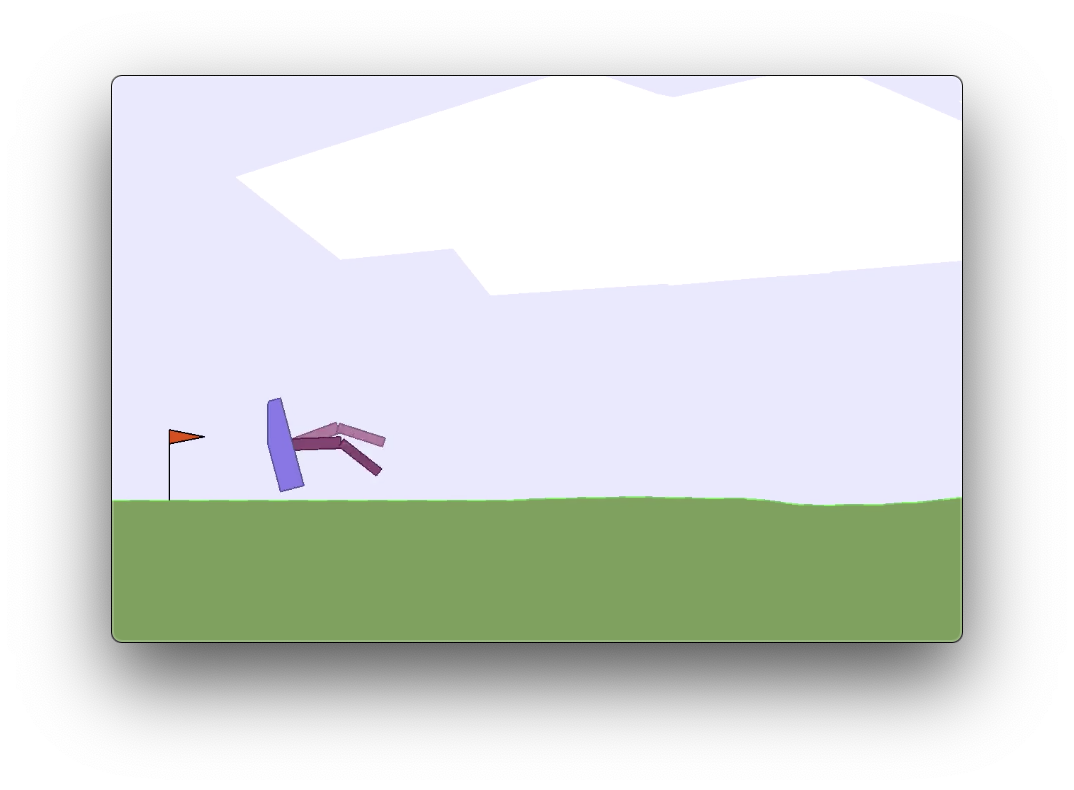
\includegraphics[scale=0.25]{images/bipedal-fall-backward.png}
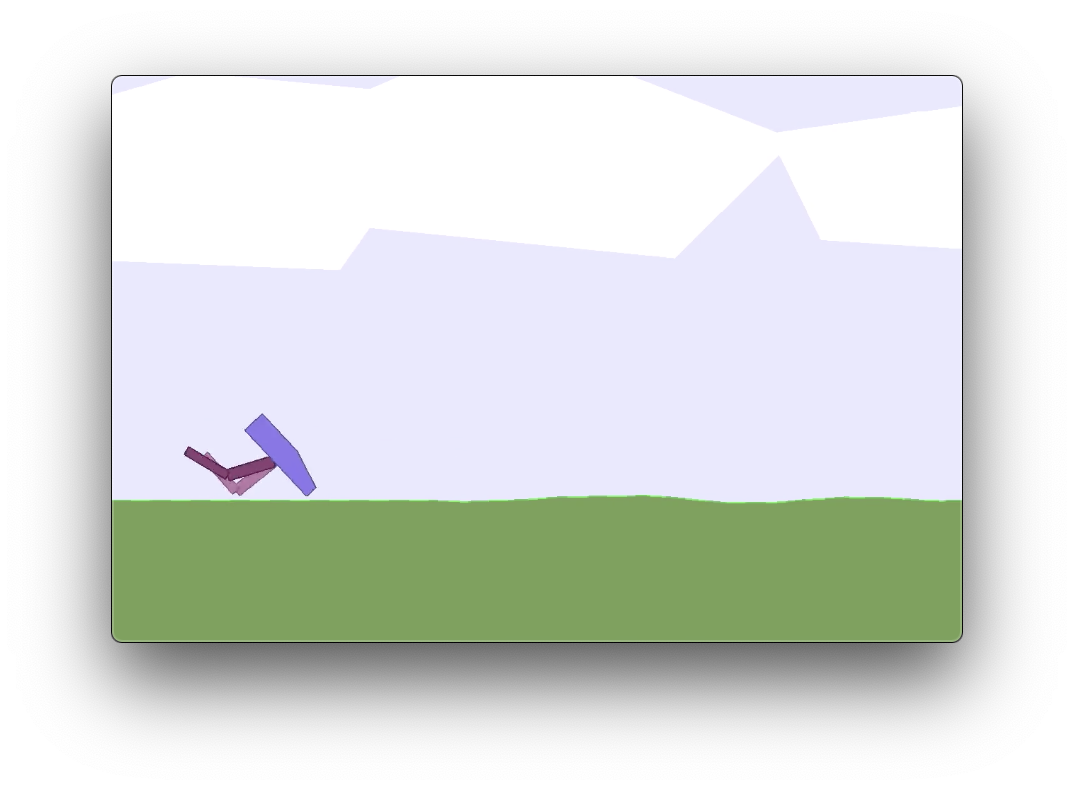
\includegraphics[scale=0.25]{images/bipedal-fall-forward.png}
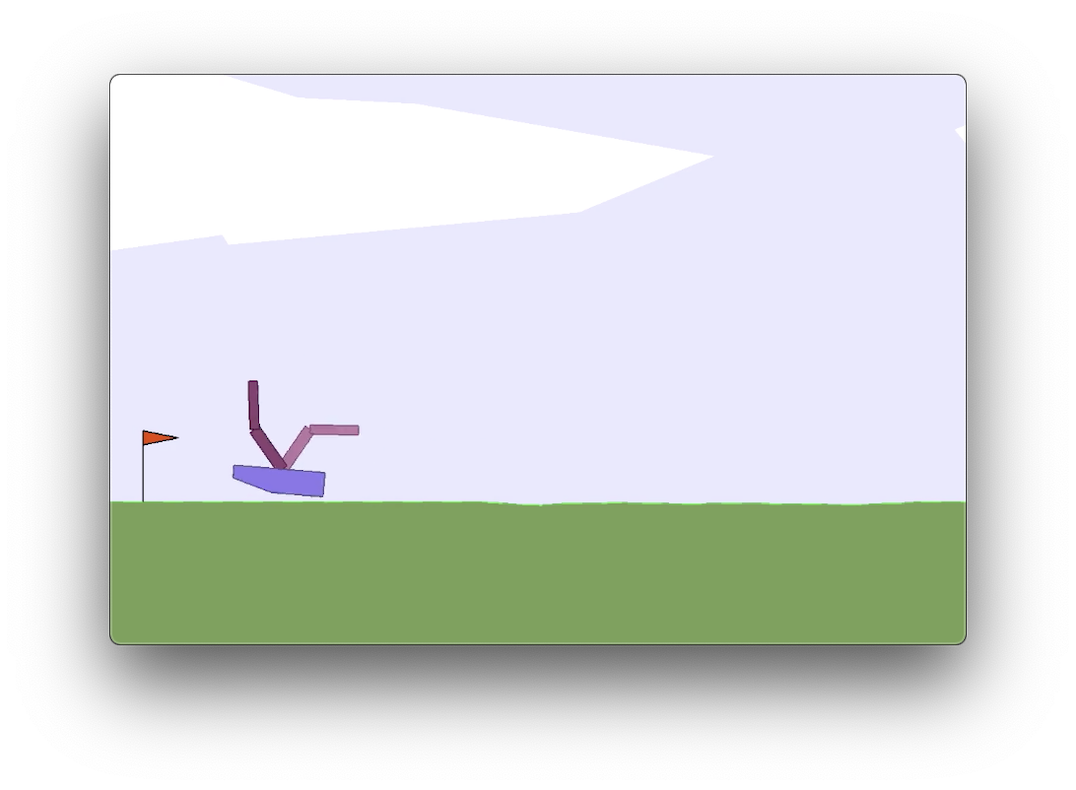
\includegraphics[scale=0.25]{images/bipedal-fall-upside-down.png}
\end{figure}

Specifically, I will be aiming to solve the BipedalWalker-v2 environment that is part of the Box2D environments on OpenAI's Gym. This environment consists of a 4-joint walker robot that is given positive reward for moving, "walking", forward. Solving is defined by OpenAI as averaging a total 300 points in 100 consecutive episodes or trials. While creating an agent that can solve the problem is the primary goal, there is a leaderboard on OpenAI that is ranked by number of episodes required before the agent solves the problem. I will compare my agent against existing results, aiming for a top result.

\section{Datasets and Inputs}
\label{sec:datasets}
The data that I'll be working with in this project is generated from the OpenAI Gym environment. For the BipedalWalker-v2 environment, the state space is a 24-dimension vector of continuous attributes, all with ranges from negative infinity to infinity. These attributes correspond to the following: hull angle speed, angular velocity, horizontal speed, vertical speed, position of joints and joints angular speed, legs contact with ground, and 10 lidar rangefinder measurements. These seem like a comprehensive set of inputs to successfully train a reinforcement learning agent.  

The other key piece of data we'll be working with is the reward given at each timestep. In this environment, a reward is given for moving forward, which can total to over 300 points for reaching the far end of the environment. If the robot falls, it gets -100. Applying motor torque costs a small amount of points, thus rewarding efficient agents.

These inputs will be used to generate the next action for the robot. The action space consists of a 4-dimensional action vector that corresponding to the motor speed of each of the 4 joints. Each speed is constrained between -1 and 1. 

\section{Solution Statement}
\label{sec:solution}
In order to solve this OpenAI Gym environment, which has both a continuous action and state space, I intend to first build a Deep Deterministic Policy Gradient agent (DDPG). I used this type of agent to solve the Quadcopter project—also a continuous action and state space environment—in the MLND's coursework. Additionally, I intend to explore modifications proposed to reduce the tendency of DDPG agents (and other Q-learning agents) to overestimate the Q-values by building a Twin Delayed Deep Deterministic Policy Gradient agent (TD3). \cite{DBLP:journals/corr/abs-1802-09477} The TD3 agent makes the following tweaks to the original DDPG algorithm. First, instead of training only one network for Q-values, TD3 takes a page out of Double-Q Learning and trains two networks to learn two Q-functions and takes the minimum Q-value between the two to reduce value overestimation. Next, it delays updating the policy until the values of the two Q-networks have converged. Finally, this technique uses a SARSA-style update for action estimates as a regularization strategy to further reduce variance. It's my hypothesis that this TD3 agent will be less brittle and will generate a solution, on average, in fewer training episodes than the DDPG agent.


\section{Benchmark Model}
\label{sec:benchmark}
As a benchmark model, I used the Vanilla Policy Gradient (VPG) algorithm implemented by OpenAI run on the Bipedal-Walker-v2 environment for 1000 epochs at 4800 steps per epoch and a maximum episode length of 1600. The gamma was set to 0.999. The rest of the configuration used default values for the experiment runner and VPG algorithm. As you can see in \ref{fig:benchmark_results}, this model was able to learn the environment and increasingly perform better, it wasn't able to "solve" the environment by scoring over 300 points in 100 consecutive episodes. Specifically, after running 3000 episodes (1000 epochs), the average total reward given over the last 99 episodes (33 epochs) was 89.91. And you can see from the chart that the agent still falls and gets penalized the -100 points. 

\begin{figure}[h]
\caption{Plot of Average Total Reward per Episode for Vanilla Policy Gradient algorithm on the Bipedal-Walker-v2 environment }
\centering
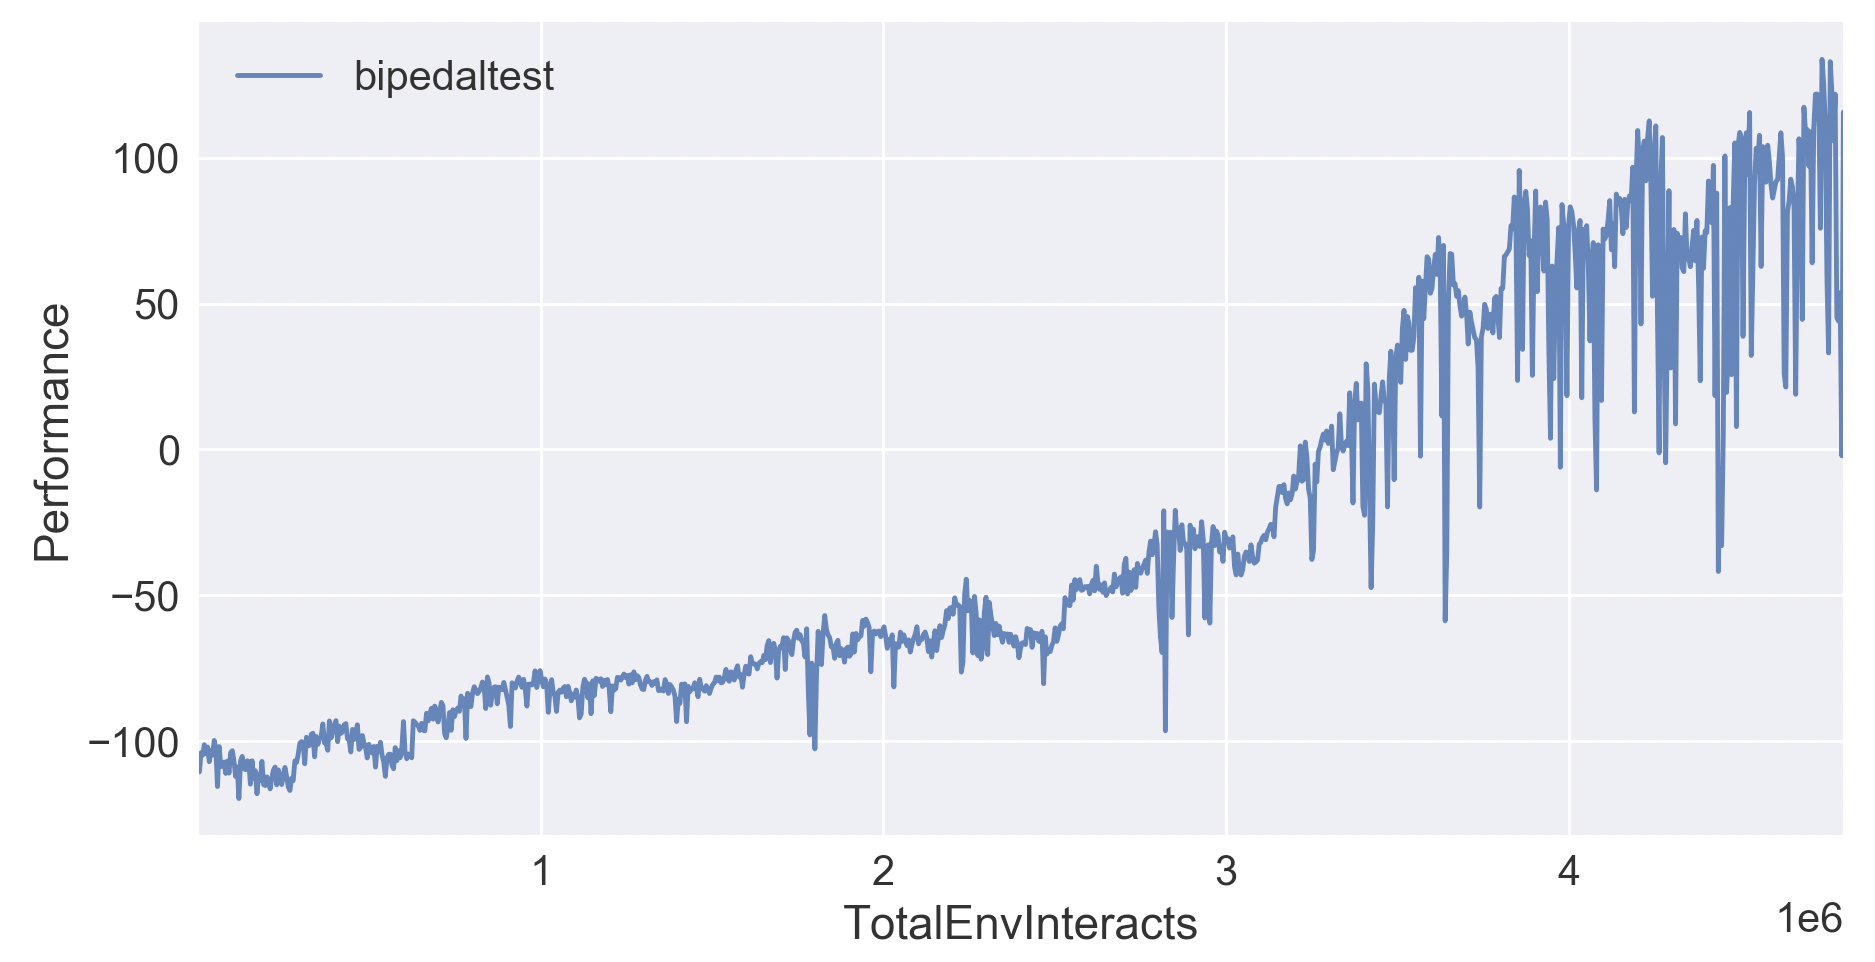
\includegraphics[scale=0.25]{images/bipedal-vpg-performance-plot.png}
\label{fig:benchmark_results}
\end{figure}

\section{Evaluation Metrics}
\label{sec:metrics}
Based on this challenge, there are two primary metrics I will use to evaluate and compare approaches. First, the total reward achieved by the trained model. For this, I'll use the average total reward across the last 100 episodes. This will be slightly lower than the final trained model as it will still be learning, but it should be consistent and give us a close enough comparison of trained agent performance. 

Additionally, we will measure and compare the number of episodes required before the agent is able to solve the problem as defined, namely averaging a total greater than 300 points in 100 consecutive episodes.

\section{Project Design}
\label{sec:design}

As described above, I plan on using a Deep Deterministic Policy Gradient agent to solve this problem. At a high-level, this approach follows the actor-critic methodology, of learning "approximations to both policy and value functions ..., where ‘actor’ is a reference to the learned policy, and ‘critic’ refers to the learned value function, usually a state-value function" \cite{Sutton:2018:RLI:3312046}. For the architecture of the the networks, I intend to start by mimicking the networks used in the original DDPG paper \cite{DBLP:journals/corr/LillicrapHPHETS15}. Specifically, I will use two hidden layers for each network, a 400 and 300 unit dense layer. For the actor, I will use a tanh activation layer. I will initialize the final layer weights and biases of both the actor and critic networks from a uniform distribution between $-3e^{-3}$ and $3e^{-3}$ to ensure the initial outputs for the policy and value estimates are near zero. I will use a $10^{-4}$ and $10^{-3}$ learning rate for the actor and critic networks respectively. I will use Adam optimization for both networks. I will use a $\gamma$ of 0.99 and a $\tau$ of 0.001. For the critic network, I will employ L2 weight decay of $10^{-2}$. Finally, I will use the Ornstein-Uhlenbeck process with $\theta = 0.15$ and $\sigma = 0.2$ for the exploration noise process. I will use a batch size of 64 and a replay buffer size of $10^{6}$. 

Once training the Deep Deterministic Policy Gradient (DDPG) agent and ideally solving the underlying OpenAI BipedalWalker-v2 environment. I will explore building a Twin Delayed Deep Deterministic Policy Gradient agent (TD3). First, I am going to duplicate the Q-network of the critic, using the same parameters and train both networks. I will then modify the critic to return the minimum Q-value to reduce value overestimation. Next, I will add a condition to only update the policy every other iteration instead of every iteration as is done in the DDPG algorithm. Finally, I'll implement the regularization technique, target policy smoothing, by adding a clipped amount of noise during the target policy update with a modified target update: $y=r+\gamma Q_{\theta'} (s', \pi_{\phi'}(s')+ \epsilon)$, where $\epsilon \sim clip(\mathcal{N}(0, \sigma), -c, c)$.

At this point, I will compare the performance of TD3 and DDPG in solving the BipedalWalker-v2 environment, specifically comparing the number of episodes required before the agent is able to solve the problem as defined, assuming both agents are able to solve the environment.

Additionally, based on some ideas in the both of the papers about these algorithms and my experience on the Quadcopter project, I intend to explore different noise strategies as well as different sizes for the hidden layers to measure the impact on these attributes of the agents.

\bibliographystyle{unsrt}  
\bibliography{references}

\end{document}
